
\chapter{Algorithms}
\label{Algorithms}
In the original study on the WISDM dataset \cite{Kwapisz:2010} employed three classification algorithms: Decision trees (J48),Logistic Regression and Multilayer Perceptron. 
all three demonstrated acceptable accuracy in distinguishing between different human movements, particularly walking, jogging, sitting, and standing. (See \ref{Table: Accuracies of Activity Recognition}) 
%J48: 89.9\% for walking; 96,5\% Jogging; 95,7\% Sitting; 93,3\% Standing
%Logistic Regression: 93,6\% ; 98\% ; 92,2\% ; 87\%
%Multilayer Perception: 91,7\%; 98,3\%; 95\% ; 91,9\%
In a subsequent study, \cite{Kant:2020}, utilized the same accelerometer data and used this time a CNN algorithm to recognize human activities using the WISDM dataset. This study demonstrated a higher degree of accuracy compared to the original study by Kwapisz, with the results presented in (insert table or numbers here).

This chapter provides a comprehensive overview of each of the four algorithms and includes a code example to illustrate its implementation.

\section{Decision trees C4.5 algorithm/J48}

%the J48, an implementation of the C4.5 algorithm In the WEKA data mining tool, is a machine learning technique that analyzes data both categorically and continuously. It is primarily used in various fields for data classification purposes, such as interpreting clinical data to diagnose coronary heart disease, classifying E-governance data, \url{https://medium.com/@nilimakhanna1/j48-classification-c4-5-algorithm-in-a-nutshell-24c50d20658e} and as seen in the original study on the WISDM dataset \cite{Kwapisz:2010} it can be used to classify human locomotion. 
%
%The C4.5 algorithm is a classification algorithm which produces decision trees based on information theory. It is an extension of Ross Quinlan’s earlier ID3 algorithm also known in Weka as J48, J standing for Java. The decision trees generated by C4.5 are used for classification, and for this reason, C4.5 is often referred to as a statistical classifier.
%\cite{Salzberg:1994}
%
%The J48 implementation of the C4.5 algorithm comes with additional features including accounting for missing values, decision trees pruning, continuous attribute value ranges, derivation of rules, etc. In the WEKA data mining tool, J48 is an open-source Java implementation of the C4.5 algorithm. J48 allows classification via either decision trees or rules generated from them.

%introduction
One of the used classification algorthims in the original WISDM dataset study is the J48, an implementation of the C4.5 algorithm In the WEKA data mining tool. This section provides a general understanding of decision trees, then introduce the C4.5 algorithm, which serves as a foundation for understanding the J48 algorithm. an at the end, a brief overview of J48.
\medskip

%decision trees 

Decision trees are recursive structures for expressing sorting rules. 
The tree usually contains tests that results with diffrent possible outcomes.
When classifying an object, we start with the root of the tree, which leads to the first test applied to our object. 
If the result of the test is a leaf, the object is assigned the class associated with that leaf.
If the root is a test, the object is evaluated against the condition of that test, and the result determines which branch of the tree to follow. Each branch represents a potential test result.
The object is thus classified by tracing out a path from the root of the decision tree to one of its leaves. \cite{Quinlan:1990}
%add example: https://developers.google.com/machine-learning/decision-forests/decision-trees
\medskip
%C4.5 

C4.5 is a classification algorithm developed in 1993 by Ross Quinlan that generates decision trees based on information theory. It is a development of older ID3 algorithm.
\url{https://medium.com/@nilimakhanna1/j48-classification-c4-5-algorithm-in-a-nutshell-24c50d20658e} 
%\cite{Salzberg:1994}

The C4.5 algorithm builds decision trees by recursively partitioning the dataset into subsets based on the values of the attributes. It selects the best attribute to split the data based on a criterion called information gain, which measures the reduction in entropy (or disorder) in the dataset.

It includes several improvements to address some of the limitations of ID3 and make it more practical and effective for real-world applications.
One of the major improvements of C4.5 is its ability to handle numeric attributes, which was not possible in ID3. C4.5 also includes techniques to handle missing and noisy data, as well as methods to generate rules from decision trees. \cite{Witten:2011}

%what is J48 
J48 is an implementation of the C4.5 algorithm that comes with additional features such as handling missing values, decision tree pruning, and generating rules from the decision tree \cite{Witten:2011}. It is an open-source Java implementation available in the WEKA data mining tool. J48 allows classification using either decision trees or rules derived from them.
%Implementation
%https://citeseerx.ist.psu.edu/document?repid=rep1&type=pdf&doi=8d509eb6e389178a426115f64a7f7213d538fca3

\section{Logistic Regression}
-- add images of the function

\url{https://www.ibm.com/uk-en/topics/logistic-regression}
%what is Logistic Regression 

Logistic Regression is a supervised machine learning algorithm used for binary classification problems such as "is Walking" or "isn’t Walking" based on a given dataset of independent variables.

the variable we want to predict (in our case Walking or not walking, sitting or not sitting...) is called the dependent variable while the variable analysed are called independent variables. 

%linear regression and logistic function

Linear regression models usually show the correlation between the wished result or the dependent variable and one or more independent variables. A solitary dependent and independent variable is termed simple linear regression, but when the number of independent variables rises, it is called multiple linear regression. 

the equation for a linear regression model with one independent variable is as follows \ref{Lin}: \cite{Jesussek:2023}
\begin{equation}
	\label{Lin}
	y = \beta_0 + \beta_1 x + \epsilon
\end{equation}

here y is the dependent or response variable and x is the independent variable. The dependent variable in this model is binary, meaning that it can only take on the values of 0 or 1, regardless of the values of the independent variables.



and in the case of using multiple independent variables, the equation is as follows \ref{Lin2}: 
\begin{equation}
	\label{Lin2}
     y = \beta_0 + \beta_1 x_1 + \beta_2 x_2 + \dots + \beta_p x_p + \epsilon
\end{equation}

in \ref{Lin} and \ref{Lin2} y is the dependent or response variable, x is the independent variable, or the factor(s) that will affect the resut, and the Beta is called the regression coefficients and it is commonly estimated via maximum likelihood estimation (MLE). 
 \cite\url{https://www.ibm.com/uk-en/topics/logistic-regression}
\begin{center}
\begin{tikzpicture}[scale=2]
	\label{LRF1}
	% Define the coordinates
	\coordinate (O) at (0,0);
	\coordinate (X) at (2,0);
	\coordinate (Y) at (0,2);
	% Draw the axes
	\draw[->] (O) -- (X) node[right] {$x$};
	\draw[->] (O) -- (Y) node[above] {$y$};
	% Plot the function
	\draw[blue,thick,domain=0:1.5] plot (\x,{-0.5+ 1.5*\x});
	% Add labels
	\node[below left] at (O) {$0$};
%	\node[below] at (X) {$x$};
%	\node[left] at (Y) {$y$};
\end{tikzpicture}
\end{center}

a linear regression equation will depending on x have infinate values (negative and positive) as you can see in  \ref{LRF1} 

since the wanted outcome is a probability, the results need to be between 0 and 1 with 0 being false and 1 True.

Here, a logistic function \ref{LFF} provides us with output values between 0 and 1 no matter what the x is. See \ref{LogisticFunction}


\begin{equation}
	\label{LFF}
f(x) = \frac{1}{1 + e^{-y}}
\quad
where
\quad
y=\beta_0 + \beta_1 x_1 + \beta_2 x_2 + \dots + \beta_p x_p + \epsilon
\end{equation}

\begin{center}
\begin{tikzpicture}
	\label{LogisticFunction}
	\begin{axis}[
		xlabel=$x$,
		ylabel=$f(x)$,
		xmin=-6, xmax=6,
		ymin=-0.1, ymax=1.1,
		samples=100
		]
		\addplot[
		domain=-6:6,
		smooth,
		thick,
		blue,
		] {1/(1+exp(-x))};
	\end{axis}
\end{tikzpicture}
\end{center}

Logistic regression is the probability of success 100\% divided by the probability of failure 1 + e\^(-y). %This is sometimes referred to as the log odds or the natural logarithm of odds.
 \cite\url{https://www.ibm.com/uk-en/topics/logistic-regression}
%Interpretation 
when using logistic regression, to decode the output as true or false (for example, is walking or isn´t walking). we classify the results by assuming that, if the output is less than 0.5 then the outcome is classified as a 0 and if it is more than 0.5 then it is classified as a 1. (with 0 being false and 1 being true).
After computing the model, it is recommended to assess the model's goodness of fit, or how well it predicts the dependent variable.
 \cite\url{https://www.ibm.com/uk-en/topics/logistic-regression}



\section{Multilayer Perceptron}
Multilayer Perceptron (MLP) is another classification algorithm used in the original study on the WISDM dataset, where it was overall the most accurate for Activity Recognition. \cite{Kwapisz:2010}. 
%structure
MLP is an artificial neural network inspired by the human brain, where a perceptron is the equivalent of a neuron. 

\begin{center}
	\begin{figure}[htbp]
		\centering
		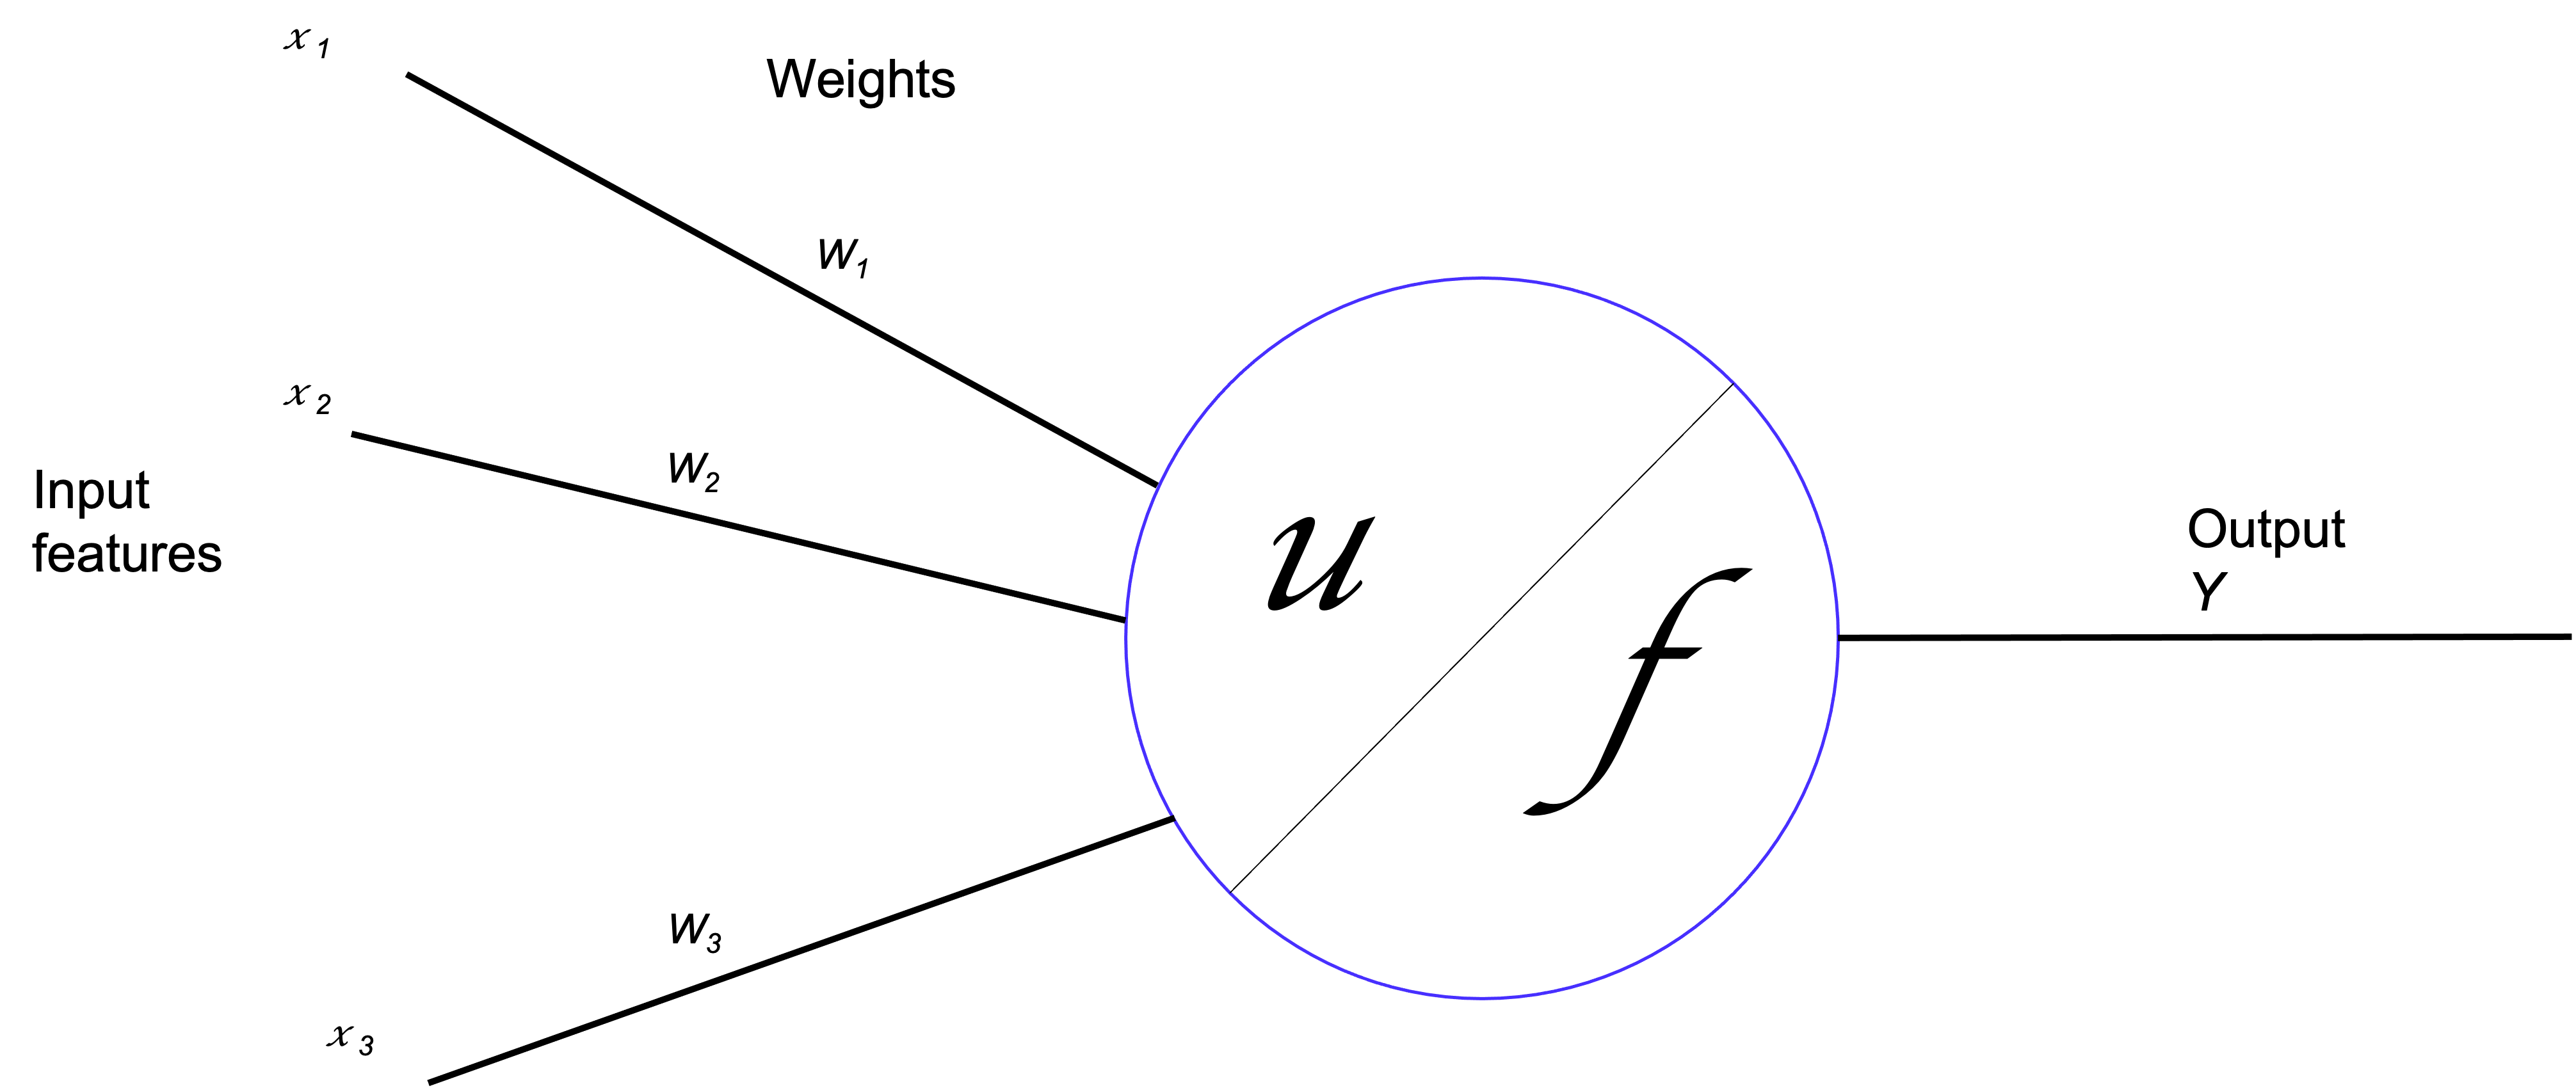
\includegraphics[width=0.75\textwidth]{Images/Scheme of a perceptron with n input features.}
		\caption{Scheme of a perceptron with n input features.}
		\label{Scheme of a perceptron with n input features.}
	\end{figure}
	
\end{center}
%--Perceptron
A perceptron (See \ref{Scheme of a perceptron with n input features.})would receive n features as input, and each of these features is associated with a weight. the perceptron will then process the input values using an input function u \ref{inputF}, which computes the weighted sum of the input features, the result of this function is then processed by an activation function \textit{f} \ref{activationF} that gives us the final output of the perceptron.\cite{Menzies:2015}. 
\begin{equation}
	\label{inputF}
	u(x) = \sum_{i=1}^{n} W_i x_i
\end{equation}
\begin{equation}
	\label{activationF}
	y = f(u(x)) = \begin{cases}
		1 & \text{if } u(x) > \theta \\
		0 & \text{otherwise}
	\end{cases}
\quad \text{where } \theta \text{ is a threshold parameter.}
\end{equation}

Note: Input features in a perceptron must be numeric so nonnumeric input must be converted before use. 



%add graph
%--Layers 
MLP in contrary to the previous classification algorithms (Logistic regression and J48), is capable of learning non-linear relationships through the use of hidden layers and activation functions. this ability to process any continuous function is made possible by using several neurons organized in at least three layers:\cite{Menzies:2015}. 

1- An input layer responsible for distributing the input features to the first hidden layer.

2- Hidden layer(s) could be one or more hidden layers of perceptrons where the first hidden layer is used as a recipient for the features distributed by the input layer, and the other hidden layers receive as inputs the output of each perceptron from the previous layer. here sigmoid functions are usually used

3- An output layer that receives as inputs the output of each perceptron of the last hidden layer. its activation function is friquently sigmoid for classification problems and the identity function for regression problems.

(https://www.elsevier.com/books/T/A/9780323855976)

\section{CNN}